\documentclass{article}
\usepackage[margin=1.0in]{geometry}
\usepackage{amsmath, amssymb, mathrsfs}
\usepackage[english]{babel}
\usepackage{graphicx}
\usepackage{enumerate}
\usepackage{tikz}
\usepackage{graphicx}


\begin{document}

\section*{Propositions}

\textit{A proposition is either True or False}

\begin{itemize}
\item may be easy or difficult to assign truth value to proposition
\item prop itself should always be precise; unambiguous
\end{itemize}

\subsection*{connectors}

\begin{align}
\text{NOT: }  \neg p &\equiv \text{ it is not the case that p} \\
\text{AND: } p \wedge q &\equiv \text{ p and q} \\
\text{OR: } p \vee q &\equiv \text{ p or q} \\
\text{IF THEN: } p \rightarrow q &\equiv \text{ if p then q / p implies q}
\end{align}

\begin{center}
\subsection*{implication}
\begin{tabular}{c c | c}
$p$ & $q$ & $p \implies q$ \\ [0.5ex]
\hline 
T & T & T \\ 
T & F & F \\
F & T & T \\
F & F & T
\end{tabular}
\end{center}

alright guess we'll just expand the table a bit

\begin{center}
\begin{tabular}{c c | c c c c}
$p$ & $q$ & $\neg p$ & $p \wedge q$ & $p \vee q$ & $p \implies q$ \\ [0.5ex]
\hline 
T & T & F & T & T & T \\ 
T & F & F & F & T & F \\
F & T & T & F & T & T \\
F & F & T & F & F & T
\end{tabular}
\end{center}

\subsection*{POP QUIZ WOO}

$$p \equiv x > 0$$
$$q \equiv y > 1$$
$$r \equiv x < y$$


\begin{table}[h!]
\centering
\begin{tabular}{c c c | c c c}
$p$ & $q$ & $r$ & $q \wedge r$ & $p \vee (q \wedge r)$ & $p \vee q$\\ [0.5ex]
\hline 
T & T & T & T & T & T\\ 
T & T & F & F & T & T\\
F & T & T & T & T & T\\
T & F & T & F & T & T\\
T & F & F & F & T & T\\
F & F & T & F & F & F\\
F & T & F & F & F & T\\ %%% this is a bad line
F & F & F & F & F & F
\end{tabular}
\caption{Note that row 7 is not actually possible.}
\end{table}

\section*{Quantifiers}

e.g., $$\text{EVERY; A; SOME; ANY; ALL; THERE EXISTS}$$

define \textit{predicate} $P(c)$ where $$C = \{c \mid c \text{ is a car}\}$$ $$ P(c) = \text{"car c has four wheels"}$$

we write the statement "for all c in C, P(c) is true" as

$$\forall c \in C : P(c)$$

e.g., for the function $f(x) = x^2$, we can write

$$\forall x \in \mathbb{R} : f(x) \geq 0$$

\newpage

\section*{More on Proofs.}

\subsection*{Direct Proof Template for proving $p \implies q$}

\textbf{Proof.}

\begin{enumerate}
\item Start by assuming that the statement claimed in $p$ is \textbf{T} 
\item Restate your assumption in mathematical terms 
\item Use mathematical and logical derivations to relate your assumption to $q$ 
\item Argue that you have shown that $q$ must be \textbf{T} 
\item End by concluding that $q$ is \textbf{T}
\end{enumerate}

\noindent\textit{Example.}

\textbf{Thm. } If $x, y \in \mathbb{Q}$, then $x + y \in \mathbb{Q}$ \\

\textbf{Proof.} 
\begin{enumerate}
\item Assume that $x,y \in \mathbb{Q}$
\item Then there are integers $a, c$ and natural numbers $b, d$ such that $x = \frac{a}{b}$ and $y = \frac{c}{d}$
\item Then $x + y = (ad + bc)/bd$
\item Since $ad + bc \in \mathbb{Z}$ and $bd \in \mathbb{N}$, $x+y$ is rational.
\end{enumerate}

\noindent\textit{Another example.}

\textbf{Thm.} If $4^x - 1$ is divisible by 3, then $4^{x+1}$ is divisible by 3 for $x \in \mathbb{R}$.

\textbf{Proof.}

\begin{enumerate}
\item Assume that $4^x-1$ is divisible by 3.
\item So $4^x-1 = 3k$ for an integer $k$, i.e. $4^x = 3k+1$
\item Observe: $4^{x+1} = 4 \cdot 4^x$. So $$4^{x+1} = 4(3k+1) = 12k + 4$$ Then $4^{x+1}-1 = 12k + 3 = 3(4k+1)$ is a multiple of 3.
\item Since it's a multiple of 3, it must be divisible by 3.
\item ayooo $q$ is \textbf{T} ***
\end{enumerate}

*** Note that we don't actually know that $4^x -1$ is divisible by 3.

\smallskip

\noindent\textit{Exercise.}

\textbf{Theorem.} For all pairs of odd integers $m, n$, the sume $m + n$ is an even integer.

\textbf{Proof.}
\begin{enumerate}
\item Assume $m$ and $n$ are both odd.
\item aighty this means that $m = 2k + 1$ and $n = 2l + 1$.
\item adding these together, we have $$m + n = 2k + 1 + 2l + 1 = 2 + 2k + 2l = 2(k + l + 1)$$
\item since $m+n$ is a multiple of 2, it is divisible by 2 and thus an even number
\item \textbf{QED}
\end{enumerate}

\subsection*{Contraposition Template for $p \implies q$}

\textbf{Proof.}
\begin{enumerate}
\item Start by assuming that the statement claimed in $q$ is \textbf{F}
\item Restate your assumption in mathematical terms
\item Use mathematical and logical derivations to relate your assumption to $p$
\item Argue that you have shown that $p$ must be \textbf{F}
\item End by concluding that $p$ is \textbf{F}
\end{enumerate}

\noindent\textit{Example}

\noindent\textbf{Theorem.} If $x^2$ is even, then $x$ is even.

\noindent\textbf{Proof.}
\begin{enumerate}
\item Assume that $x$ is odd.
\item Then $\exists k \in \mathbb{Z} : x = 2k + 1$
\item Then $x^2 = 2(2k^2 + 2k) + 1$
\item This means $x^2$ is 1 added to a multiple of 2, so it's odd.
\item $x^2$ is odd so the proof is over lol
\end{enumerate}

\noindent\textit{Exercise}

\noindent\textbf{Theorem.} If $r$ is irrational, then $\sqrt{r}$ is irrational.

\noindent\textit{Proof.}
\begin{enumerate}
\item Let's assume $\sqrt{r}$ is rational.
\item So $\exists a,b \in Z : \sqrt{r} = \frac{a}{b}$
\item What happens when we square it? $$\sqrt{r}^2 = (\frac{a}{b})^2$$ $$r = \frac{a^2}{b^2}$$ $a$ and $b$ are both integers, so $r$ must be rational
\item So it's clear that $r$ is not irrational in this case (it is rational).
\item unnecessary restatement of concluding $p$ is \textbf{F}
\end{enumerate}

\subsection*{Equivalence: sort of a sidenote} 
\begin{center}
IF AND ONLY IF
\end{center}
$$p \iff q$$

This just means you have to prove the implication \textbf{both ways}.

\subsection*{Contradictions}

e.g.,
\begin{center}
$1=2$;     $n^2 < n \text{ for } n \in \mathbb{N}$;     $| x | <  x$;     $p \wedge \neg p$
\end{center}

Wowie these look \Large\textbf{FISHY}\normalsize don't they?

\noindent\textbf{Proof Template}
\begin{enumerate}
\item To derive a contradiction, assume that $p$ is \textbf{F}
\item Restate your assumption in mathematical terms
\item Derive a \LARGE\textbf{FISHY}\normalsize statement?a contradiction that must be false
\item Thus, the assumption in step 1 is false, and $p$ is \textbf{T}
\end{enumerate}

\noindent\textit{Exercise}

\textbf{Theorem}. Let $a, b$ be integers. Then $a^2 - 4b \neq 2$

\textbf{Proof.}
\begin{enumerate}
\item Say $a^2 - 4b = 2$
\item Then $$a^2 = 2 + 4b = 2(1+2b)$$ $$a = \sqrt{2}\sqrt{1+2b}$$
\item $\sqrt{2}$ is irrational, so $a$ must be irrational, so it's not an integer. but $a$ is an integer. \LARGE\textbf{FISHY.}\normalsize
\item alright so we must have $$a^2 -4b \neq 2$$
\end{enumerate}

\subsection*{Proofs about Sets}

Let's look at $A \cup (B \cap C) = (A \cup C) \cap (A \cup C)$

\smallskip

\def\firstcircle{(90:.6cm) circle (1.cm)}
\def\secondcircle{(210:.6cm) circle (1.cm)}
\def\thirdcircle{(330:.6cm) circle (1.cm)}

\begin{minipage}{.2\textwidth}
\begin{tikzpicture}
  \begin{scope}[fill opacity=0.5]
    \clip \firstcircle;
    \fill[cyan] \firstcircle;
  \end{scope}
  \begin{scope}[fill opacity=0.5]
    \clip \secondcircle;
    \fill[yellow] \thirdcircle;
  \end{scope}
  \draw \firstcircle node[text=black,above] {$A$};
  \draw \secondcircle node [text=black,below left] {$B$};
  \draw \thirdcircle node [text=black,below right] {$C$};
  \end{tikzpicture}
\end{minipage}
=
\begin{minipage}{.2\textwidth}
\begin{tikzpicture}
  \begin{scope}[fill opacity=0.5]
    \fill[cyan] \firstcircle;
    \fill[cyan] \thirdcircle;
  \end{scope}
  \begin{scope}[fill opacity=0.5]
    \fill[yellow] \thirdcircle;
    \fill[yellow] \secondcircle;
  \end{scope}
  \draw \firstcircle node[text=black,above] {$A$};
  \draw \secondcircle node [text=black,below left] {$B$};
  \draw \thirdcircle node [text=black,below right] {$C$};
  \end{tikzpicture}
\end{minipage}
-
\begin{minipage}{.2\textwidth}
\begin{tikzpicture}
  \begin{scope}[fill opacity=0.5, even odd rule]
    \clip \firstcircle;
    \clip \thirdcircle;
    \fill[red] \secondcircle;
  \end{scope}
  \draw \firstcircle node[text=black,above] {$A$};
  \draw \secondcircle node [text=black,below left] {$B$};
  \draw \thirdcircle node [text=black,below right] {$C$};
  \end{tikzpicture}
\end{minipage}
  
\newpage

\section*{Induction}

\textbf{Template}

\begin{enumerate}
  \item Show $P(1)$
  \item Assume $P(n)$
  \item Show $P(n) \implies P(n+1)$
\end{enumerate}

%%%%%%%%%%%%%%
% 5 Feb 2017 %
%%%%%%%%%%%%%%

\newpage

\section*{More Proof-y Things}

\subsection*{Well-Ordering Principle}

\textit{Any non-empty set of natural numbers has a minimum element.}

\smallskip

This is important because induction follows form well ordering. e.g.

Take some predicate $P(n)$. If $P(1)$, and $P(n) \implies P(n+1)$, then $P(n)$ for $n \geq 1$.

\noindent\textbf{Proof.} Suppose $P(1)$ and $P(n) \implies P(n+1)$ for $n \geq 1$.

Assume $P(n)$ false for some values of $n$, with $n*$ representing the smallest counterexample for $P(n)$. Here, $n* > 1$ because $P(1)$ is true. 

Given this assumption, $n*-1$ is not a counterexample because $n*$ is the smallest counterexample, so $P(n* -1)$ is true.

But since $P(n*-1)$ is true, we must have $P(n*-1) \implies P(n*)$. So we have a contradiction. Therefore $P(n)$ is true for all $n \geq 1$.

\noindent\textbf{An example}

$$n < 2^n \text{ for } n \geq 1$$

\noindent\textbf{Proof.}

\noindent \textit{Induction.}  

$P(1)$ is true because $1 < 2$. Assume $P(n)$ true. Then

$$n + 1 \leq n + n = 2n \leq 2 \cdot 2^n = 2^{n+1}$$

So $P(n+1)$ is true and therefore $P(n)$ is true.

\smallskip

\noindent \textit{Well-ordering}

Assume that there is an $n \geq 1$ such that $n \geq 2^n$. Let $n*$ be the minimum example of this, so $n* \geq 2^n$. 

We know $1 < 2^1$, so $n* \geq 2$, which gives $\frac{1}{2}n* \geq 1$. So

$$n* - 1 \geq n* - \frac{1}{2}n* = \frac{1}{2}n* \geq \frac{1}{2} \cdot 2^{n*} = 2^{n*-1}$$

which \large means \normalsize that $n* -1$ is a \large smaller \normalsize counterexample! ooOOoOOOO.

\bigskip

\noindent \large \textbf{Harder} \normalsize

\noindent Prove $\sum_{i=1}^{n} \frac{1}{\sqrt{i}} \leq 2n$.

\noindent \textbf{Proof.}

$P(1)$: $1 \leq 2\cdot \sqrt{1}$ is true.

Assume $P(n)$. Then for $P(n+1)$ we have

$$\sum_{i=1}^{n+1} \frac{1}{\sqrt{i}} \leq 2\sqrt{n+1}$$

We can use the assumption of $P(n)$ to rewrite this

\begin{align*}
  \sum_{i=1}^{n+1} \frac{1}{\sqrt{i}} &= \sum_{i=1}^{n} \frac{1}{\sqrt{i}} + \frac{1}{\sqrt{n+1}}\\
  &\leq 2\sqrt{n} + \frac{1}{\sqrt{n+1}}
\end{align*}

And here we use a \textit{Lemma.} $2\sqrt{n} + \frac{1}{\sqrt{n+1}} \leq 2\sqrt{n+1}$

Which we prove by contradiction:

\begin{align*}
  2\sqrt{n} + \frac{1}{\sqrt{n+1}} &> 2 \sqrt{n+1} \\
  2 \sqrt{n(n+1)} + 1 &> 2(n+1) \\
  4n(n+1) &> 4(n+1)^2 \\
  4n &> 4n + 4
\end{align*}

Wow fishy.

\textit{Back to the proof:}

\begin{align*}
  \sum_{i=1}^{n+1} \frac{1}{\sqrt{i}} &\leq 2\sqrt{n} + \frac{1}{\sqrt{n+1}} \\
  &\leq 2\sqrt{n+1}
\end{align*}

So $P(n)$ is true for all $n \geq 1$.

\bigskip

\noindent \textbf{Prove} $n^2 \leq 2^n \text{ for } n \geq 4$

$$4^2 = 16 \leq 2^4 = 16$$

Assume that $n^2 \leq 2^n$ and that $2n + 1 \leq 2^n$. Then $$(n+1)^2 = n^2 + 2n + 1 \leq 2^n + 2n + 1\leq 2^n + 2^n = 2^n+1$$

\bigskip

\subsection*{the tile problem}

Can you tile a $2^n \times 2^n$ patio missing one of the center squares, using only the corner shaped tile?

let $P(n) := $ the $2^n \times 2^n$ grid minus a center square can be $L$-tiled.

Suppose $P(n)$ is \textbf{T}. WELL. The $2^{n+1} \times 2^{n+1}$ patio can be separated into four $2^n \times 2^n$ patios.

Think about adding the center $L$ to this first. Then all four of the subtiles were/are missing a corner square. Thus we can revise the original claim to be

$Q(n) :$

\begin{centering}
  (i) the $2^n \times 2^n$ grid missing a center square can be $L$-tiled. \\
  (ii) the $2^n \times 2^n$ grid missing a corner square can be $L$-tiled.
\end{centering}

So add base cases and complete the proof.





\bigskip

\noindent \subsection*{Different Problem} $P(n) : n^3 < 2^n$ for $n \geq 10$

Suppose $P(n)$ is true. Consider $P(n+1) : (n+1)^3 < 2^{n+2}$ ??

\begin{align*}
  (n+2)^3 &= n^3 + 6n^2 + 12n +8 \\
  &< n^3 + n n^2 + n^2 n + n^3 \\
  &< 4n^3 < 4 \cdot 2^n = 2^{n+2}
\end{align*}

so $$P(n) \implies P(n+2)$$

We can have two base cases to cover all cases---$P(10)$ and $P(11)$ are both true.

\section*{THE FUNDAMENTAL THEOREM OF ARITHMETIC}

\textbf{SUPPOSE $n \geq 2$. Then (i) $n$ can be written as a product of prime factors, and (2) the representation of $n$ as a product of primes is unique.}

We could use $P(n)$: $n$ is a product of primes. But this is hard. So let's use $$Q(n) : P(2) \wedge P(3) \wedge P(4) \wedge \cdots P(n)$$

\textbf{Proof.} Q(1) claims 2 is a product of primes, which is true.

Assume that $Q(n)$ is true, so each of $2, 3, \dots , n$ are prime products. Since we know $Q(n)$, to prove $Q(n+1)$, we just need to show that $n+1$ is a product of primes. There are some possible cases here:

\begin{itemize}
  \item    $n+1$ is prime. Fin. 
  \item  $n+1$ not prime, so $n+1 = kl$ where $2 \leq k,l \leq n$ 
\end{itemize}

In the second case, we know that $P(k)$ and $P(l)$ are both true, so $k$ and $l$ are both products of primes. Thus $kl$ is a product of primes, so $n+1$ is a product of primes. $Q(n+1)$ is true for all $n \geq 2$.

\subsection*{Strong Induction}

To prove $P(n) \forall n \geq 1$ by strong induction, use induction to prove the \textit{stronger} claim that $Q(n) : $ each of $P(1), P(2), \dots , P(n)$ are true.

\bigskip

\begin{tabular}{c c  c}
$ $ & Ordinary Induction & Strong Induction\\ [0.5ex]
\hline 
  Base Case & Prove $P(1)$ & Prove $Q(1) = P(1)$  \\ 
  Induction Step & $P(n) \implies P(n+1)$ & $Q(n) = P(1) \wedge \dots \wedge P(n) \implies P(n+1)$ 
\end{tabular}

\newpage

\section*{Induction is Important}

\subsection*{Applications of Inudction}

\begin{itemize}
    \item Tournament rankings \\
    \item Greedy or recursive algorithms \\
    \item Games of strategy
\end{itemize}

\noindent\textbf{Equal Pile Nim.}

\begin{centering}
$P(n)$: Player 2 can win the ame that starts with $n$ pennies in each row.
\end{centering}

Player 2 can always return the game ot smaller equal piles. If player 2 wins the smaller game, Player 2 wins the larger game. Strong Induction!

\subsection*{In General}

Recursive functions must have some base case, and a recursive progression that leads to the base case.p

\newpage

\section*{TREES}


\includegraphics[width=\textwidth]{baby-animals-tree-trunk-bears-cubs-brown-cutest-zoo-1920x1080.jpg}

\subsection*{Exercise 7.12 \normalsize Give recursive definition}

\textbf{(a) } $S = \{3^0, 3^1, 3^2, \dots\}$

$$1 \in \mathbb{S}$$
$$x \in \mathbb{S} \rightarrow 3\cdot x \in \mathbb{S}$$

\textbf{(b) } $S = \{$all binary strings that are palindromes$\}$

$$\{\},0,1 \in S$$
$$x \in S \implies 0x0 \in S \wedge x \in S \implies 1x1 \in S$$

\textbf{(c) } $S = \{$all strings of matched parentheses$\}$ 

$$\{\} \in S$$ $$x,y \in S \implies [x]y \in S$$

\subsection*{Rooted Binary Tree}

\textbf{Definition.}

The empty tree $\epsilon$ is an RBT

If $T_1, T_2$ are disjoint RBTs with roots $r_1$ and $r_2$, then linking $r_1$ and $r_2$ to a \textit{new} RBT with root $r$

\subsection*{Structural Induction}

\begin{itemize}
  \item Base Cases are True
  \item For every constructor rule, show: if P is T for the known parents, THen P is T for children
  \item By structural induction, conclude that P(s) is T for all s in S
\end{itemize}

































\newpage

\section*{Number Theory Stuff.}

\subsection*{Some Basics}

\subsection*{GCD}

Euclid's algorithm

\subsection*{Bezout's Identity}

\textbf{Theorem.} $\gcd(m,n)$ is the smallest positive integer linear combiantion of $m$ and $n$:

$$\gcd(m,n) = mx + ny \qquad \text{for } x,y \in \mathbb{Z}$$

\subsection*{Crazy Facts about the GCD}

\begin{enumerate}[(i)]
  \item $\gcd(m,n) = \gcd(m,\text{rem}(n,m))$
  \item Every common divisor of $m, n$ divides $\gcd(m,n)$
  \item For $k \in \mathbb{N}$, $\gcd(km, kn) = k\cdot \gcd(m,n)$
  \item If $\gcd(l,m) = 1$ and $\gcd(l,n) = 1$, then $\gcd(l,mn) = 1$
  \item If $d \mid mn$ and $\gcd(d,m) = 1$, then $d \mid n$
\end{enumerate}


\bigskip

\begin{align*}
  5^2 &\equiv 1 \mod 3 \\
  (5^2)^{1007} &\equiv 1 \mod 3 \\
  5 \cdot (5^2)^{1007} &\equiv 5 \equiv 2 \mod 3
\end{align*}

\subsection*{Modular Division things}

Suppose $ac \equiv bc \mod d$. Then $a \equiv b \mod d$ if $\gcd(c,d) = 1$.







\section*{GRAPHS}

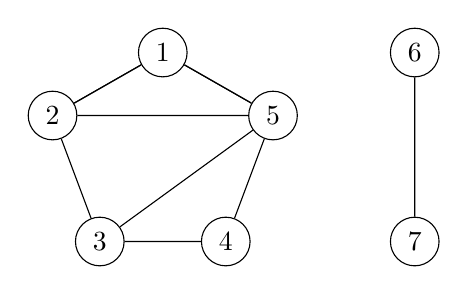
\begin{tikzpicture}
  [scale=.8,auto=left,every node/.style={circle}] %,fill=blue!20}]
  \node[draw, circle] (n1) at (3,8) {1};
  \node[draw, circle] (n2) at (1.25,7)  {2};
  \node[draw, circle] (n3) at (2,5)  {3};
  \node[draw, circle] (n4) at (4,5) {4};
  \node[draw, circle] (n5) at (4.75,7)  {5};
  \node[draw, circle] (n6) at (7,8)  {6};
  \node[draw, circle] (n7) at (7,5)  {7};

  \foreach \from/\to in {n1/n2,n1/n5,n5/n1,n1/n2,n2/n5,n2/n3,n3/n4, n4/n5, n3/n5, n6/n7}
    \draw (\from) -- (\to);

\end{tikzpicture}









\newpage

\section*{COUNTING}

This is what discrete math is all about.

  Say you have three kinds of things and you organize them into groups of three. how many possible groups? There are 10.
  But what happens when you scale up? gets a lot harder.

\textbf{Sum Rule.} $N$ objects of two types: $N_1$ of type 1 and $N_2$ of type 2. Then $N = N_1 + N_2$.

$$|\{A_1 A_2 \dots A_n \}| = |A_1||A_2|\cdots|A_n|$$

Example: 10 runners; how many possible top 3 finishes? $|\{FST\}| = 10 \times 9 \times 8 = 720$








\end{document}
